\documentclass[a4paper,10.5pt]{article}
\usepackage{mathtools}
\usepackage{listings}
\usepackage[utf8x]{inputenc}
\usepackage[left=2.2cm,top=2cm,right=2.2cm,bottom=2cm,nohead,nofoot]{geometry}
\setlength{\footskip}{25pt}
\renewcommand{\footnoterule}{%
  \kern -3pt
  \hrule width \textwidth height 0.5pt
  \kern 2pt
}
\usepackage{marginnote}
\usepackage{pgfgantt}
\usepackage{rotating}
\usepackage{pdflscape}
\title{Random Number Generation using Genetic Programming\ \ \ \  \ \ \      Interim Report}
\author{Philip Leonard}
\date{}
\begin{document}
\maketitle
\begin{abstract}
This is the Interim Report for the project; `Random Number Generation using Genetic Programming' by Philip Leonard, supervised by Dr David Jackson (primary supervisor) and Professor Paul Dunne (secondary supervisor).\\\\
\textbf{Keywords:} Genetic Programming/Program (GP), Pseudo Random Number Generator (PRNG), Random Number Generator (RNG), Entropy, Single Node Genetic Programming/Program (SNGP).
\end{abstract}
\section{Completed Work}
\subsection{GP Implementation}

I first completed the Genetic Programming implementation around November 2013. Upon doing test runs I realised that it was taking much longer than I had first anticipated. By using the clock function in C (which calculates CPU time), I calculated the running times of the main procedures and narrowed down the bottle neck, which happened to be the fitness function for finding the occurrences of binary subsequences. I substituted the brute force matching algorithm with the KMP (Knuth Morris Pratt) algorithm, an  efficient finite automaton based pattern matching algorithm. By doing this I was able to reduce the running time drastically, however this still remains the bottle neck (highest order operation) in the program.

While the running time of the GP implementation remains slow in my eyes, the results of the runs are promising. To begin with I was surprised that solutions needed more generations to find a solution than I originally anticipated. But upon considering that the search space for this problem is relatively large, and that Koza defines a solution as a RNG with extremely high entropy I came to accept this.

In \cite[p.6]{kozarng}, Koza says that he finds a solution in 14 generations. Some runs of my implementation may only take so long (as seen in the example run \& fig \ref{gp-ss}), but they can take around 30 to 60 generations to find one. As Koza says in \cite[p.6]{kozarng}, entropy slowly improves in the region of 27.800 to 27.900 bits, and as this method isn't driven by hill climbing, the entropy value fluctuates.\\


\begin{center}
RNG Tree (27.991340 bits of entropy) 

+/+-/-/J3-**/-/J3-+J1/J23/+3+**//J233+J33%J+/J32-**/J33+J/J2+1J23JJ31
\end{center}

\begin{figure}[!h]
\centering
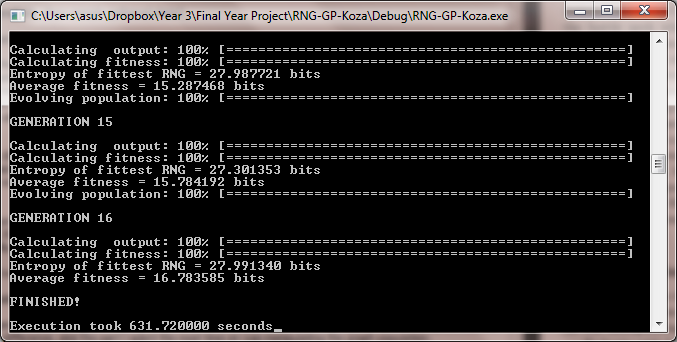
\includegraphics[width=120mm]{gp-ss.png}
\caption{GP implementation example run screenshot}
\label{gp-ss}
\end{figure}

The time that can be seen in fig \ref{gp-ss} is measured in CPU time (the accumulative time the thread has a hold on the CPU), and not real time. Otherwise this would reflect the speed of the CPU and not necessarily the efficiency of the program. After being generally pleased with the outcomes of the GP implementation I moved onto the SNGP implementation.

\subsection{SNGP Implementation}

The next step was to implement the SNGP program. Having completed the GP implementation, I was able to quickly complete this due to there similarities. The main difference, and the part I spent the most time on was manipulating the graph population. 

To begin with I implemented the program where I updated every node in the graph. Once I had this running correctly, I then went about implementing an update list method of determining the nodes that needed to be updated by recursively finding the parent(s) of the mutated node. Using this dynamic programming method, the run time of the program drastically improved. 

From the runs that I have tested the program with it seems that SNGP is a faster method for finding high entropy RNGs than standard GP is. I was also surprised that this method was taking more hill climbing smut operations than I first anticipated, but I then realised that I was giving as an input an inordinately large fitness sum level for it to achieve (POP\_SIZE * 27.90). I then changed the implementation slightly to include a stop condition of a single RNG fitness threshold, and lowered the fitness sum target (as having every tree in the graph being of such a high fitness was proving near impossible).

After doing this the SNGP approach began producing good results, and although still taking quite a number of smut operations, it was executing far quicker than the GP approach (as can be seen in \ref{sngp-ss} below).

\begin{center}
RNG Tree (27.984177 bits of entropy) 

/*+*-3--*+/+1J3/3013/30---*+/+1J3/3013/300+-* 
//+1J31+1J///+1J312\%/302++%+1J+/+1J3/ 
30+-*//+1J31+1J///+1J312\%/302\%1J+1J 
\end{center}

\begin{figure}[!h]
\centering
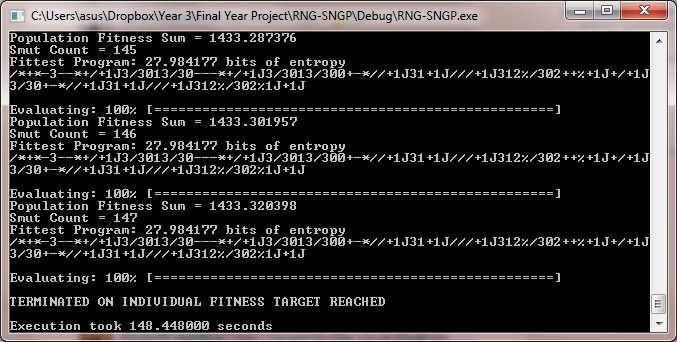
\includegraphics[width=120mm]{sngp-ss.png}
\caption{SNGP implementation example run screenshot}
\label{sngp-ss}
\end{figure}

\subsection{TRNG \& C rand() Test program}
The final part of the implementation phase was to implement the program to test both the Random.org TRNG and the C rand() function. Random.org supplies an API for which a sequence of Random bits produced by there instruments can be requested over the web. I implemented the program so that 16384 bits are requested over HTTP and then saved to a file on the users hard disk. This file is then read into a char* and the entropy is then tested in the exact same way as that of a RNG in the GP and SNGP approaches. The program then outputs the entropy data to the user which can then be collected.

The program also allows the user to check how many bits they have left in the quota (for the current ip address), out of 1,000,000 bits which Random.org provides for free.

The program can also test the C rand function. The program seeds the C rand function with the current system time and then requests 16384 bits from the rand function in order to populate a char*. The entropy is then tested in the exact same way and the results are shown to the user. See fig \ref{trng-ss} for a example runs of both.

\begin{figure}[!h]
\centering
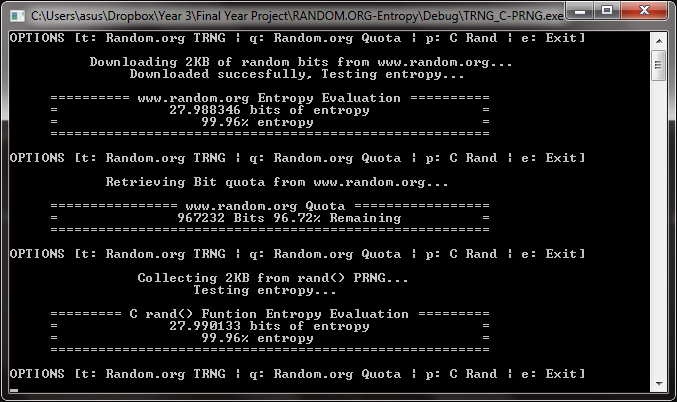
\includegraphics[width=120mm]{trng-ss.png}
\caption{TRNG \& C rand() test program screen shot}
\label{trng-ss}
\end{figure}

\section{Remaing Work}

Th remaining work to be completed is as follows;\\

\noindent - Gather data from multiple runs of each method\\
- Compare all approaches using test criteria described in the design document \\
- Finally, give demonstration and write dissertation based on findings\\\\
By referring to the Gantt chart in fig 4, we can see that the project is about 1 month ahead of schedule. The next stage is to gather and compare the data from all approaches.

\begin{thebibliography}{1}

\bibitem{kozarng}
  John R. Koza, 
  \emph{Evolving a Computer Program to Generate Random Numbers Using the Genetic Programming Paradigm}. 
  Stanford University, 
  1991.

\end{thebibliography}
\begin{sidewaysfigure}

\centering
\begin{ganttchart}[y unit title=0.4cm,
y unit chart=0.5cm,
vgrid,hgrid, 
title label anchor/.style={below=-1.6ex},
title height=1,
bar/.style={fill=gray!50},
bar/.append style={fill=gray!100},
bar incomplete/.append style={fill=gray!50},
incomplete/.style={fill=white},
progress = today,
today = 23,
bar height=0.7,
group right shift=0,
group top shift=.6,
group height=.3,
group peaks height =.2,
milestone/.append style={fill=gray!50}
]
{1}{34}
%labels
\gantttitle{Final Year Project}{34} \\
\gantttitle{Sep}{2} 
\gantttitle{Oct}{4} 
\gantttitle{Nov}{4} 
\gantttitle{Dec}{4} 
\gantttitle{Jan}{4} 
\gantttitle{Feb}{4} 
\gantttitle{Mar}{4} 
\gantttitle{Apr}{4} 
\gantttitle{May}{4} \\
%tasks
\ganttbar{Research}{1}{6} \\
\ganttgroup{Specification}{2}{4} \\
\ganttbar{Write Specification}{2}{4} \\
\ganttgroup{Design}{5}{10} \\
\ganttbar{Plan Design}{5}{5}\\
\ganttbar{Write Design Document}{6}{9}\\
\ganttbar{Plan Presentation}{9}{9}\\
\ganttbar{Give Design Presentation}{10}{10} \\
\ganttmilestone{Implementation Documentation Complete}{10}\\
\ganttgroup{Implementation}{11}{26} \\
\ganttbar{Implement Koza's PRNG GP}{11}{18}\\
\ganttbar{Implement SNGP Approach}{19}{23} \\
\ganttbar{Compare GP vs SNGP}{24}{26}\\
\ganttmilestone{Implementation Complete}{26} \\
\ganttgroup{Demonstration}{27}{28} \\
\ganttbar{Write/Plan Demonstration}{27}{27} \\
\ganttbar{Give Demonstration}{28}{28} \\
\ganttgroup{Dissertation}{29}{34} \\
\ganttbar{Plan Dissertation}{29}{29}\\
\ganttbar{Write Dissertation}{30}{34} \\
\ganttmilestone{Project Completed}{34} \\

%relations
\ganttlink[link type=dr]{elem2}{elem4} 
\ganttlink[link type=dr]{elem4}{elem5}
\ganttlink[link type=dr]{elem4}{elem6}
\ganttlink[link type=dr]{elem5}{elem8}
\ganttlink[link type=dr]{elem6}{elem7}
\ganttlink[link type=dr]{elem7}{elem8} 
\ganttlink[link type=dr]{elem8}{elem10} 
\ganttlink[link type=dr]{elem10}{elem11}
\ganttlink[link type=dr]{elem10}{elem12}
\ganttlink[link type=dr]{elem11}{elem12}
\ganttlink[link type=dr]{elem12}{elem13} 
\ganttlink[link type=dr]{elem13}{elem15}
\ganttlink[link type=dr]{elem15}{elem16}
\ganttlink[link type=dr]{elem16}{elem18}
\ganttlink[link type=dr]{elem18}{elem19}
\ganttlink[link type=dr]{elem19}{elem20}

\end{ganttchart}

\caption{Gantt Chart - Work plan}
\end{sidewaysfigure}
\end{document}